\chapter{Image segmentation with Deep Learning}
In this chapter, we will look at the problem of image segmentation and the state of the art regarding segmentation and object detection using Deep Learning. We will look at both semantic and instance segmentation.

Semantic segmentation of images is one of the key problems in the field of computer vision. It is about making dense predictions inferring labels at the pixel level, assigning a class to each pixel with its enclosing object \cite{Garcia-Garcia2017}. Taking it a step further, we get to instance segmentation, where we want to associate the classes with a physical instance of an object. 

Both semantic and instance segmentation can be seen as giving us an understanding of an image at a higher level. This fine-grained control of an image greatly helps with scene understanding which is becoming more and more relevant with the increasing number of applications, such as self-driving cars and augmented reality. 

We can see an example in \autoref{fig:segmentation} where we see the difference between the two approaches. In the middle photo, all the chairs have the same classification, as chairs. In the right photo, we see that the chairs now are classified as chairs, but with a different class for each of them. We can see that instance segmentation is the combination of both object detection and semantic segmentation.

\begin{figure}[H]
	\centering
	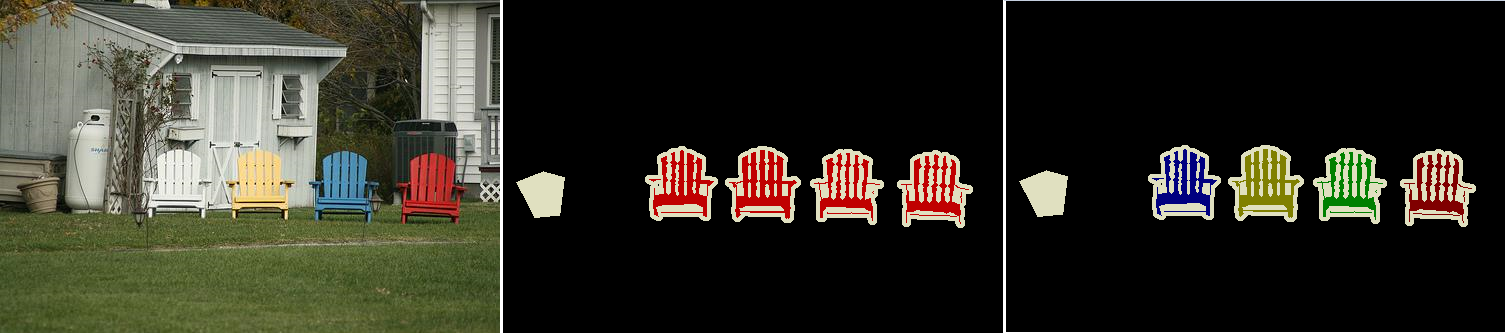
\includegraphics[width=0.8\linewidth]{fig/se.png}
	\caption{Left: input image. Middle: Semantic segmentation. Right: Instance segmentation. \cite{PASCALVOC2012}}
	\label{fig:segmentation}
\end{figure}


\section{Neural networks}
To get a deeper understanding of how neural networks perform segmentation of images, we need to take a look at the fundations behind them and how they operate.

Neural networks are a computational model that shares som properties with the animal brain in which simple units called neurons are working in parallel with no centralized control unit \cite{Patterson2017}. The primary means to long-term information storage is in the weights between the units and updating them is the primary way the network learns new information.

A network is defined by the number of neurons, number of layers and the connections between the layers. One of the easiest architectures to understand is the feed-forward multilayer architecture viewed in \autoref{fig:feed-forward}. It is a neural network with an input layer, one or more hidden layers and an output layer. The input layers feeds input, in the form of vectors, to the rest of the network. The number of neurons at the input layer often reflects the size of the input vector.

\begin{figure}[H]
	\centering
	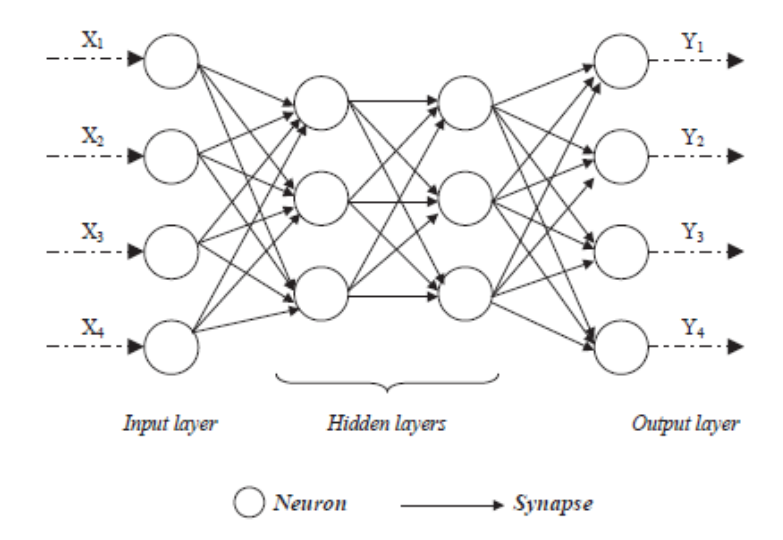
\includegraphics[width=0.6\linewidth]{fig/feedforward-neural-network.png}
	\caption{Structure of a multilayer feed forward network. \cite{Zangeneh2011}}
	\label{fig:feed-forward}
\end{figure}

\subsection{Artificial neurons}
Each layer consist of one or more artificial neurons, also called nodes. An artificial neuron is a mathematical representation of a biological neuron and consist of inputs with weights and bias, a transfer function and an activation function. The weights are what scales, either amplifying or decreasing, the input to the node. The bias is a constant scalar value per layer that is added to ensure that at least some of the nodes in the layer are activated, that is, forwarding a non-zero value to the next layer. The transfer function takes the weighted sum of the input variables and transfers it to the activation function. The activation functions are scalar-to-scalar functions that defines the output of the node based in the inputs, weights and bias. A model of an artificial neuron compared to a real one, can be seen in \autoref{fig:artificial-neuron}. 


\begin{figure}[H]
	\centering
	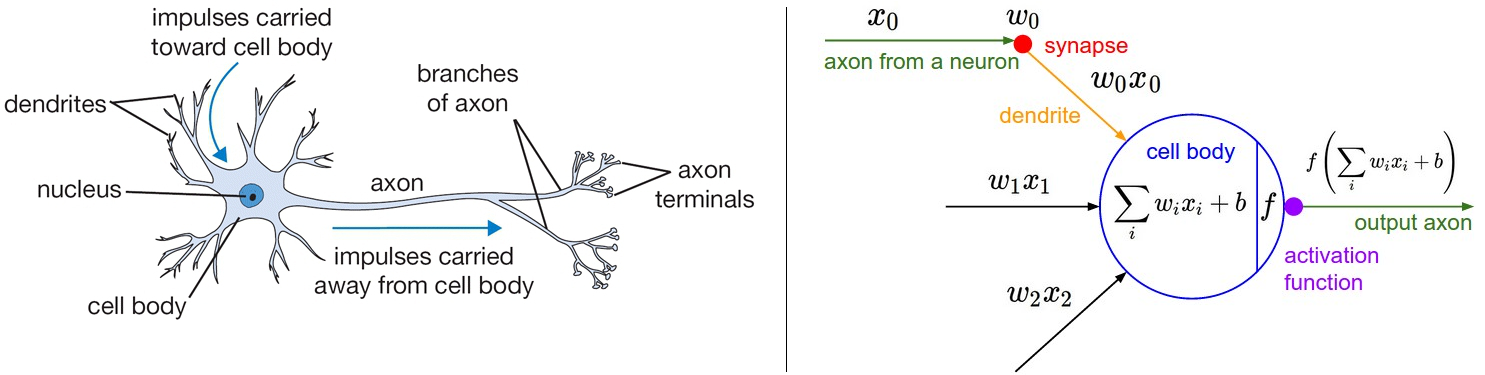
\includegraphics[width=\linewidth]{fig/artificial-neuron.png}
	\caption{Structure of a real neuron compared with an artificial one. \cite{Li}}
	\label{fig:artificial-neuron}
\end{figure}

\subsubsection*{Activation functions}

The use of activation functions in the hidden layers add the ability for the network to learn non-linear functions. We will now take a look at some of the usefull activations functions that are used today.

\subparagraph*{Sigmoid}

The sigmoid activation function has a characteristic "S"-shaped curve and can take variables of near infinite range and convert them to values between 0 and 1. It is good at reducing outliers and extreme values in the dataset. Expressed mathematical as:

\begin{equation}
a = \sigma(x) = \frac{1}{1+\exp(-x)}
\end{equation}


\subparagraph*{Tanh}

A trigonometric hyperbolic function. Tanh can normalize input to the range of -1 to 1 and can therefore deal with negative numbers better than the Sigmoid. Expressed mathematically as:

\begin{equation}
a = \sigma(x) = \tanh(x)
\end{equation}


\subparagraph*{Rectified Linear}

Rectified Linear only activates a node if it is above some threshold. When the input raises above the threshold it has a linear relation to \autoref{eq:relu}. Nodes that use the rectifier are called Rectified Linear Unit or ReLU. 

\begin{equation}
\label{eq:relu}
a = \sigma(x) = \max(0, x)
\end{equation}


ReLUs are the state-of-the-art because of their proven usefulness in many situations and their ability to train better in practice than sigmoids. ReLU does not have the so-called problem of vanishing gradients either. Vanishing gradients is a problem that occurs when using gradient-based methods (EXPLAINED LATER) for learning, where large changes in the value of parameters from the early layers, does not have a big effect on the output, making the network lose its ability to learn. The reason for this happening is that some activation functions, such as sigmoids or tanh, forces the input space into small regions. 

While removing the problem of vanishing gradients, ReLU introduces another one and that is the problem of "dying ReLU" \cite{Li}. This is a problem that occurs when a large gradient passes through the neuron causing the weight update to be so large that it causes the neuron to never activate again, that means that the gradient passing through the neuron will be forever zero.


\subsection{Training}
There are different forms of learning such as supervised, where we show the network what the correct answer is. Unsupervised, where the network itself decides how to label the data and reinforcement learning, where the network does not get to know the answer but learns by reward or punishment. We will only focus on supervised learning in this paper as this is the type of learning we use when doing image segmentation.

In supervised learning, the network learns by training on a set of inputs and desired outputs. As inputs are passed through the network and outputs are generated, it learns by adjusting weights and biases causing some neurons to become smaller and some to become larger. The larger a neuron's weight is, the more it affects the network and vice versa.

By adjusting the weights and biases, the network reduces the errors, also called loss. The loss is defined by some loss function that quantifies the correctness of the output from the network in regards to the ground truth. By using a loss function we reclass the learning problem as an optimization problem, where we try to minimize the loss.

The most common algorithm for the weight adjustment in neural networks is called \emph{backpropagation}.


\subsubsection*{Backpropagation Learning}
When the output from a neural network produces a large loss, we need to update the weights accordingly. A problem with multilayer neural networks, however, is that there are many weights connecting an input with an output, so it becomes difficult knowing what weights that affect the output. We need a clever way of finding what specific weight that contributes to the output. This is the problem backpropagation tries to solve. A high level understanding of backpropagation is that we use the chain rule to iteratively calculate the gradients for each layer. The steps of the algorithm is as follows:

\begin{enumerate}
	\item Initialize network with random weights
	\item Loop trough the training examples
	\item Compute the network output for the current training example
	\item Compute the loss with the loss function.
	\item Compute the weight update for the output layer with the weight update rule:
	$$
		W_{j,i} \leftarrow W_{j,i} + \alpha \times \alpha_j \times \Delta_i
	$$
	
	Where 
	$$
		\Delta_i = Err_i \times g'(input\_sum_i)
	$$
	
	and $g'$ is the derivative of the activation function
	
	\item Loop trough all the layers in the network all the way to the input layer and:
	\item Compute the error at each layer with the propagation rule:
	$$ 
		\Delta_j \leftarrow g'(input\_sum_i)\sum_{i}W_{j,i}\Delta_i
	$$
	
	\item Update the weights leading in to the hidden layer with the update rule:
	
	$$ 
		W_{k,j} \leftarrow W_{k,j} + \alpha \times \alpha_k \times \Delta_j
	$$
	
\end{enumerate}

The term $\alpha$ is the learning rate, and belongs to the family of what we call \emph{Hyperparameters} in machine larning.

\subsubsection*{Hyperparameters}
The hyperparameters are what we tune to make the network train faster and better. The selection of these parameters are done to ensure that our network does not \emph{overfit} or \emph{underfit} the data. We say that our model is overfitted if it fits our training data too well but does not generalize enough over the entire dataset. We say our model is underfitted if it generalizes too much and is not able to fit the training set. The terms are illustrated in \autoref{fig:overfit-underfit}. In the left image we see that the model does a bad job at approximating the function, it is underfitted. In the middle image we see that the model approximates the function well. In the right image we see that the model fits the training samples very good, but does a bad job at approximating the function, the model is overfitted.

\begin{figure}[H]
	\centering
	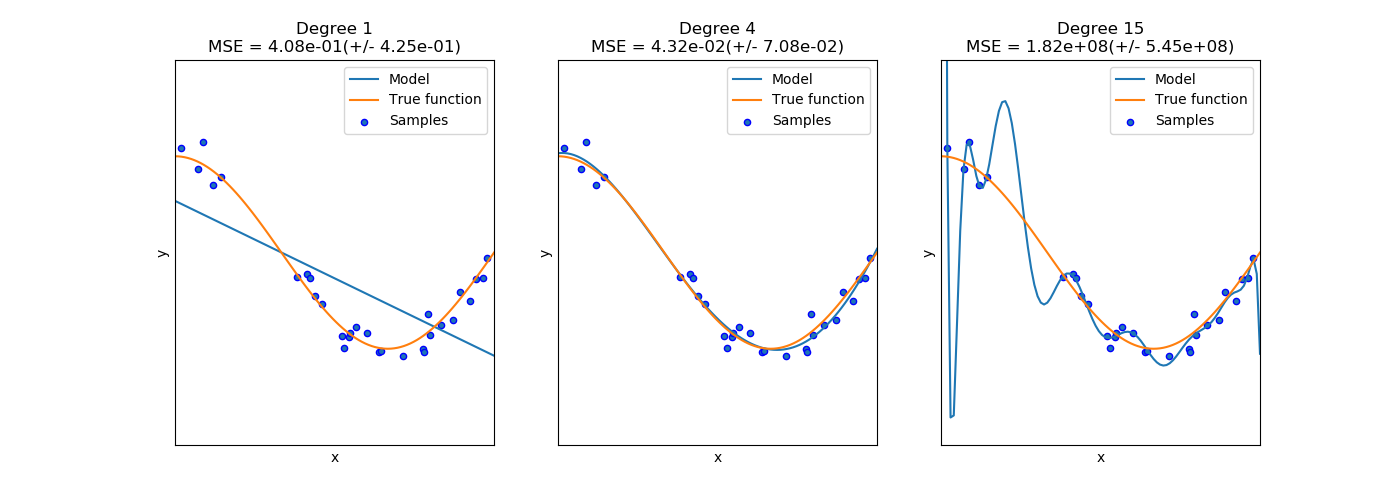
\includegraphics[width=\linewidth]{fig/overfit-underfit.png}
	\caption{Left: Underfitted model. Middle: Appropriate fit. Rigth: Overfitted model. }
	\label{fig:overfit-underfit}
\end{figure}
The learning rate affects the amount we adjust the parameters during training. A large learning rate will make our parameters take large steps, thus saving time, but can cause us to overshoot the minimum of our loss function causing us to never find a minimum. A small learning rate causes us to take smaller steps and should help us reach the minimum, but can take a very long time to do so.

Another important hyperparameter is \emph{regularization}. Overfitting often occurs when some weights have become very large and regularization is about reducing the effects of the large weights in the network. The perhaps most common form of regularization is L2 and is often implemented as the term $\frac{1}{2}\lambda w^2$ that we add to the weights \cite{Li}. Another regularization, introduced in \cite{Srivastava2014} is \emph{dropout}. Dropout works by randomly dropping some of the neurons during training causing it to train on a "thinned" version of the net. Dropout has shown  major improvements over other regularization tehniques \cite{Srivastava2014}.

\section{Convolutional neural networks}
Fully connected multilayer neural networks take inputs as a one-dimensional vector. When using an image as input, these vectors become very large. The reason for this is that we represent each pixel in the image as one value in the vector. If we are working with color images represented with 3 channels of RGB information, each of these also needs to be mapped. For a single 200x200 image this means $200 \times 200 \times 3 = 120000$ connections in only the first layer. This illustrates how bad the fully connected neural networks scale.

Convolutional neural networks, or CNNs, tackle the scaling problem by assuming inputs as images and model them as three-dimensional objects with image width, image height and color channels as the dimensions. At a high level, the architecture consist of an input layer, convolutional layers, pooling layers and fully-connected layers \cite{Patterson2017}. 

\subsection{Convolutional layers}
The convolutional layers, or CONV layers, are the core building blocks of a CNN. The layers consist of a set of learnable filters also called kernels. Each of the filters are small in regards to width and height but are always the same size as the input in regards to depth. The filter is applied to the input by sliding, or \emph{convolving}, the filter accross the width and height of the input. At each position, the dot product between the filter and the input is calculated. The output is a two dimensional map that is called \emph{activation map}. This process is illustrated in \autoref{fig:convolution}. For each of the filters in the CONV layer we get such a map and stack them in the depth direction, this in turn represents the output of the layer. 

\begin{figure}[H]
	\centering
	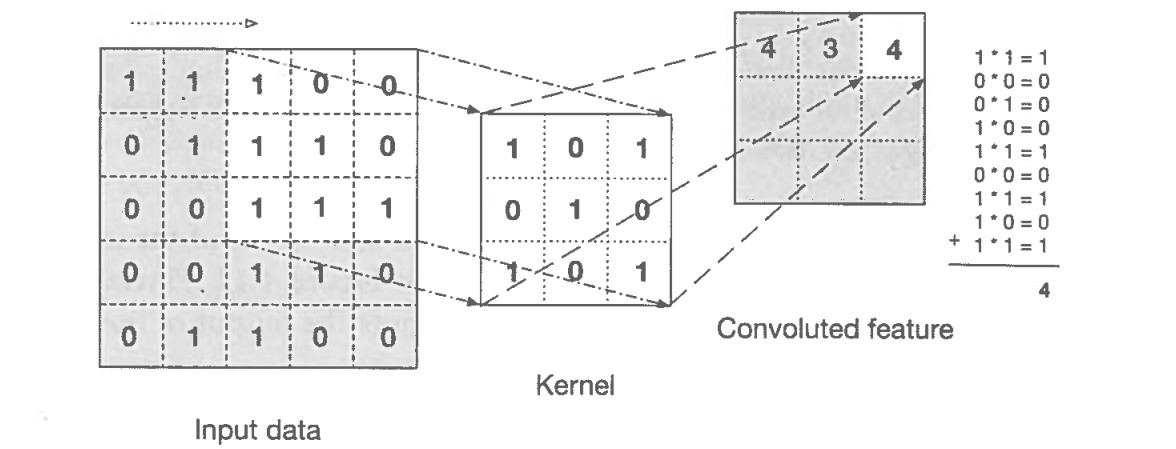
\includegraphics[width=\linewidth]{fig/convolution.png}
	\captionsource{The convolution step.}{\citeauthor{Patterson2017}\cite{Patterson2017}}
	\label{fig:convolution}
\end{figure}

The network will learn filters that causes the node to activate when certain visual features are seen, for instance an edge. Deeper into the network we will se filters that become more global in term of the input and recognizes nonlinear combinations of features. An example of what the filters look like in a deep CNN can bee seen in \autoref{fig:filters} where we see filters learned in the first convolutional layer in an eight layer network \cite{Krizhevsky2012}.

\begin{figure}[H]
	\centering
	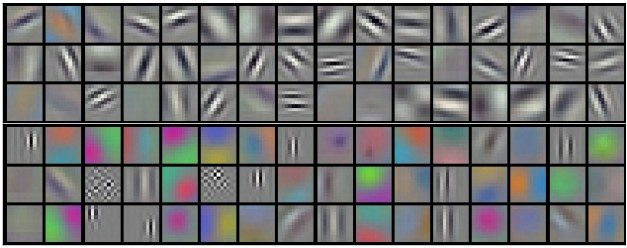
\includegraphics[width=\linewidth]{fig/filters.png}
	\captionsource{96 learned filters in the first convolutional layer. }{\citeauthor{Krizhevsky2012}\cite{Krizhevsky2012}}
	\label{fig:filters}
\end{figure}
%  Local connectivity
If we imagine that we freeze the filter as it is convoluted accross the input, a single step and its calculation, can be viewed as the output from a neuron. The activation map then represents a sheet of neurons with each of the neurons looking at a small part of the input, not knowing anything about the rest of the image. This feature is called \emph{local connectivity} and is an important part of how the network keeps the number of parameters smaller then a regular neural network. All the neurons in the sheet also share parameters, since it is the same filter that did the calculation. This is the concept of \emph{shared paramters} and is the other important part of how CNNs keep the number of paramters low.

\subsection{Pooling layers}
Another way to reduce the number of parameters in the network, is the use of pooling layers. Pooling layers essentially reduces the input size by downsampling the input with different pooling functions. The most common operation is \emph{max pooling} with a 2x2 filter with a stride of 2 that reduces the size by two in the height and width dimension \cite{Li}. 






















